\chapter{The Gamma Framework and Exact Asymptotic Scaling}\label{ch:gamma}

Chapter~\ref{ch:persist} reduced a persistent orbit to the pair \((\gamma_n,L_n)\). This chapter makes that reduction exact: a one-step law computes the next fibre from \(\gamma\) and the exponents alone (Theorem~\ref{thm:onestep}); a finite-state closure shows that every persistent orbit is eventually class-periodic and therefore scales exactly (Theorem~\ref{thm:closure}); and the carry mechanism is analysed until its structure is explicit (Theorems~\ref{thm:window}--\ref{thm:qcarry}). Throughout, \(x=\gamma L^2/g\) is a persistent state with \(G(x)=g>1\), \(L=\prod_pp^{e_p}\), \(o_p=\ord_g(p)\), \(w=\gamma+1\), \(h=\gcd(g,w)\), \(b'=g/h\). A \emph{carry} is a step with \(L_{n+1}\neq L_n\), \(r=L_{n+1}/L_n\); a \emph{plateau} is a run of steps with \(r=1\).

\begin{remark}[The scaling question and its answer]\rec{F.T48}\scope{C}\label{rem:T48}
The natural conjecture, that every orbit eventually satisfies \(x_{n+3}=4x_n\) with \(x_n=s_n^2t_n/g\), \(t_n\in\{1,2,3\}\), holds for \(G_\infty=1\) (Theorem~\ref{thm:regimeI}) and for the regimes of Theorems~\ref{thm:Pg} and~\ref{thm:Pstar}, but it is not a statement about all orbits: the orbit of Theorem~\ref{thm:eight} below has \(x_{n+3}/x_n\) taking eight different values forever. The correct universal statement is Theorem~\ref{thm:closure}: every orbit eventually satisfies \(x_{n+P}=\rho^2x_n\) for some period \(P\) and some integer \(\rho\ge2\), with \((P,\rho)\) depending on the orbit.
\end{remark}

\section{The one-step law}

\begin{theorem}[One-step law]\rec{F.T49}\scope{C}\label{thm:onestep}
Let \(x=\gamma L^2/g\) be persistent. Put \(\sigma'=L\prod_pp^{\lfloor\vv_p(w/h)/2\rfloor}\). Then \(x'=C(x)=wL^2/g\) and
\[
\Dx(x')=\{d\mid\sigma':\ d\ge2,\ d\equiv1\ (\mathrm{mod}\ b')\}.
\]
The point \(x'\) is persistent iff every \(d\) in this set is \(\equiv1\ (\mathrm{mod}\ g)\). In that case \(L'=\mathrm{lcm}\,\Dx(x')\) is a multiple of \(L\), \(r=L'/L\) is an integer with \(r\mid\prod_pp^{\lfloor\vv_p(w/h)/2\rfloor}\) and \(r^2\mid w\), and
\[
\gamma'=w/r^2.
\]
\end{theorem}
\begin{proof}
\(x'=x+L^2/g=(\gamma+1)L^2/g=wL^2/g\). As \(\gcd(L,g)=1\), the reduced form has numerator \((w/h)L^2\) and denominator \(b'=g/h\). Now \(d^2\mid(w/h)L^2\) iff \(2\vv_p(d)\le\vv_p(w/h)+2e_p\) for all \(p\), iff \(\vv_p(d)\le e_p+\lfloor\vv_p(w/h)/2\rfloor\), iff \(d\mid\sigma'\). If every such \(d\equiv1\ (\mathrm{mod}\ g)\) then \(g\mid G(x')\); and \(G(x')\mid G(x)=g\) by Theorem~\ref{thm:mono}; hence \(G(x')=g\). Conversely persistence requires \(g\mid d-1\) for all \(d\in\Dx(x')\). \(L\mid L'\) from \(\Dx(x)\subseteq\Dx(x')\), and \(L'\mid\sigma'\) gives \(r\mid\prod p^{\lfloor\vv_p(w/h)/2\rfloor}\). Finally \(\gamma'=gx'/L'^2=wL^2/L'^2=w/r^2\), an integer by Theorem~\ref{thm:gamma}(a).
\end{proof}

The theorem makes the dynamics a computation on residues: the only information about the exponent \(e_p\) that enters is the set \(\{p^k\bmod g:0\le k\le e_p+s'_p\}\). This is the ``residue machine'' used for all certificates in this volume (Appendix~\ref{app:algo}).

\section{The eight-step orbit and the failure of a uniform period}

\begin{theorem}[The eight-step orbit at \(g=11\)]\rec{F.T50}\scope{C}\label{thm:eight}
Let \(S_k=2^2\cdot3^{3+k}\cdot5^4\) and \(x=tS_k^2/11\). For every \(k\ge0\):
\begin{enumerate}[label=(\roman*),nosep]
\item \(L(tS_k^2/11)=S_k\) for \(t=1,\dots,8\); \(L(9S_k^2/11)=3S_k=S_{k+1}\); and \(G=11\) throughout;
\item the orbit of \(C\) from \(x_0=67500^2/11\) is \(x_{8k+j}=(j+1)S_k^2/11\) (\(j=0,\dots,7\)); hence \(x_{n+8}=9x_n\), with \(\gamma\)-cycle \(1\to2\to\dots\to8\to1\) and one 3-carry per 8 steps;
\item \(R(x_{8k+j})=7+2k\), so \(R(x_{n+8})=R(x_n)+2\);
\item \(x_{n+3}/x_n\) takes the eight values \(3/2,\ 8/5,\ 7/4,\ 2,\ 5/2,\ 18/7,\ 27/8,\ 4\), each once per period.
\end{enumerate}
\end{theorem}
\begin{proof}
\(g=11\) is prime and \(w\le9<11\), so \(h=1\), \(b'=11\). Modulo 11: \(3\) has order 5 and \(H=\langle3\rangle=\{1,3,4,5,9\}\) (the quadratic residues); \(2\notin H\), \(4=3^4\in H\), \(8=2\cdot4\notin H\), \(5\equiv3^3\), \(12\equiv1\). By Theorem~\ref{thm:onestep} the fibre of \(wS_k^2/11\) is \(\{d\mid S_k\cdot\mathrm{sqrtpart}(w):d\equiv1\ (\mathrm{mod}\ 11)\}\).

\emph{\(L\) is attained.} Write \(d=2^a3^b5^c\); its residue is \(2^a3^{b+3c}\). Since \(2\notin H\) and \(4\in H\), the residue lies in \(H\) only for \(a\in\{0,2\}\) (for \(a\le2\)), and \(d\equiv1\) iff \(5\mid b+3c\) (\(a=0\)) or \(5\mid4+b+3c\) (\(a=2\)). For \(b=3+k\) the congruence \(c\equiv-(3+k)3^{-1}\ (\mathrm{mod}\ 5)\) has a solution \(c\in\{0,\dots,4\}\), so \(\vv_3=3+k\) is attained. \(5^43^i=3^{12+i}\equiv1\) needs \(i\equiv3\ (\mathrm{mod}\ 5)\): \(i=3\le3+k\), so \(\vv_5=4\) is attained; a suitable \((b,c)\) with \(a=2\) attains \(\vv_2=2\). These congruences are periodic in \(k\bmod5\), so \(L(S_k^2/11)=S_k\); for \(t\in\{1,2,3,5,6,7\}\), \(\sigma'=S_k\), so \(L\) cannot grow.

\emph{No absorption for \(t=1,\dots,8\).} For \(t\in\{4,8\}\), \(\sigma'=2S_k\) has \(\vv_2=3\); a divisor with \(\vv_2=3\) would need \(2^33^i5^c\equiv1\), i.e. \(8\in H\), which is false.

\emph{The 3-carry at \(t=9\).} \(\sigma'=3S_k\) has \(\vv_3=4+k\); \(d=3^{4+k}5^c\) with \(5\mid4+k+3c\) is solvable, so \(L'=3S_k\) and \(\gamma'=9/9=1\).

\emph{\(G=11\).} \(12=2^2\cdot3\mid S_k\) and \(12\equiv1\ (\mathrm{mod}\ 11)\) with \(12-1=11\), so \(G\mid11\); every \(d\equiv1\ (\mathrm{mod}\ 11)\), so \(G=11\).

\emph{Counts.} \(d=2^a3^b5^c\equiv1\) forces \(a\in\{0,2\}\); for each \(a\) and each \(c\) exactly one residue class of \(b\bmod5\) works, and the classes for \(c=0,\dots,4\) are distinct, so \(\sum_c\#\{b\le B:b\equiv b_c\}=B+1\) with \(B=3+k\). Hence \(R=2(4+k)-1\), the \(-1\) removing \(d=1\). Item (iv) is exact arithmetic on the closed form of (ii).
\end{proof}

\begin{figure}[t]
\centering
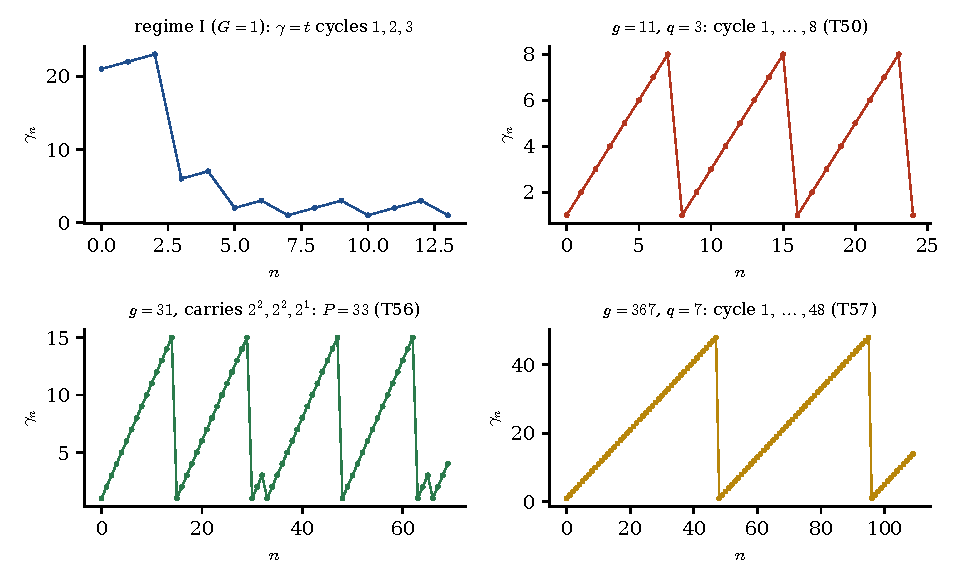
\includegraphics[width=0.97\linewidth]{figs/fig_gamma.pdf}
\caption{The arithmetic state cycles \(\gamma_n\) of four orbits, computed from the residue machine and cross-checked against direct iteration of \(C\): regime~I (\(G=1\), cycle \(1,2,3\)); \(g=11\), \(q=3\) (cycle \(1,\dots,8\), Theorem~\ref{thm:eight}); \(g=31\) with carries \(2^2,2^2,2^1\) (period 33, Theorem~\ref{thm:odometer}); \(g=367\), \(q=7\) (cycle \(1,\dots,48\), Theorem~\ref{thm:qcarry}). Each reset to \(\gamma=1\) is a carry.}\label{fig:gamma}
\end{figure}

\begin{figure}[t]
\centering
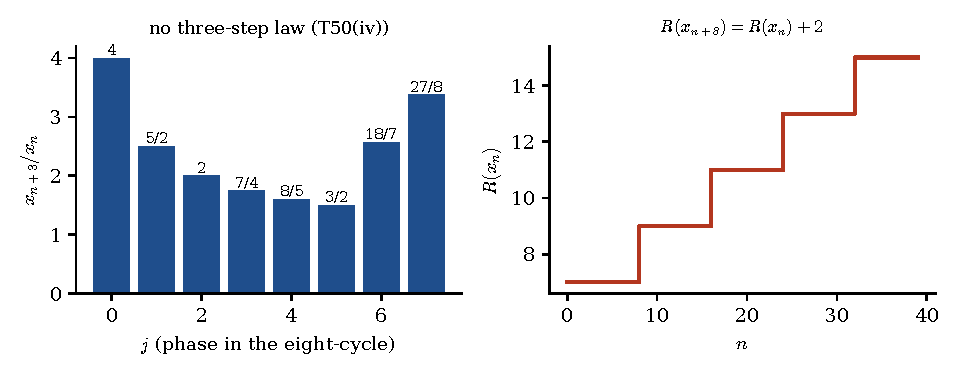
\includegraphics[width=0.97\linewidth]{figs/fig_ratios.pdf}
\caption{The eight-step orbit of Theorem~\ref{thm:eight}, from exact iteration of \(C\). Left: the eight values of \(x_{n+3}/x_n\) over one period; no single three-step law holds (Remark~\ref{rem:T48}). Right: the fibre multiplicity \(R(x_n)\), which rises by 2 every eight steps.}\label{fig:ratios}
\end{figure}

The orbit of Theorem~\ref{thm:eight} is the first of a family with arbitrarily large cycle \(1,\dots,q^2-1\) (Theorem~\ref{thm:qcarry}); it shows concretely that the period \(3\) of regime~I is a feature of \(G_\infty=1\), not of persistence as such (Remark~\ref{rem:T48}).

\section{Finite-state closure and exact scaling}

For a prime \(p\nmid g\) and \(e\ge0\) define the \emph{class}
\[
c_p(e)=\begin{cases}e,&e\le o_p-2,\\ (o_p-1)+\big((e-(o_p-1))\bmod o_p\big),&e\ge o_p-1,\end{cases}
\]
so classes are \(0,1,\dots,2o_p-2\). The class of a persistent state is \((\gamma,(c_p(e_p))_p)\), with \(c_p=0\) when \(e_p=0\).

\begin{lemma}[Class lemma]\label{lem:class}
The class of \(C(x)\), the carry vector \(\Delta_p=e'_p-e_p\), and persistence of \(C(x)\) are functions of the class of \(x\).
\end{lemma}
\begin{proof}
By Theorem~\ref{thm:onestep} the data of the step are \(w,h,b'\), \(s'_p=\lfloor\vv_p(w/h)/2\rfloor\) (functions of \(\gamma\)) and, for each \(p\), the residue set \(\{p^k\bmod g:0\le k\le e_p+s'_p\}\). If \(e_p\ge o_p-1\), that set is all of \(\langle p\rangle\) whatever \(e_p\) is; if \(e_p<o_p-1\) it depends on \(e_p\) exactly. The new exponent is \(e_p+\Delta_p\) with
\[
\Delta_p=\max\{j\in[0,s'_p]:\ p^{e_p+j}a\equiv1\ (\mathrm{mod}\ b')\text{ for some }a\in\mathcal A_{-p}\},
\]
where \(\mathcal A_{-p}\) is the set of residues of divisors of \(\sigma'/p^{\vv_p(\sigma')}\) (\(j=0\) is always attained since \(\Dx\subseteq\Dx'\)). This depends on \(e_p\) only through \(e_p\bmod o_p\) (saturated) or exactly (unsaturated). The persistence test, ``all \(d\equiv1\ (\mathrm{mod}\ b')\) are \(\equiv1\ (\mathrm{mod}\ g)\)'', is a statement about the same residue sets. Finally \(c_p(e+\Delta)\) depends only on \(c_p(e)\) and \(\Delta\).
\end{proof}

\begin{theorem}[Class closure and exact scaling]\rec{F.T51}\scope{C}\label{thm:closure}
\begin{enumerate}[label=(\alph*),nosep]
\item \emph{Closure principle.} If two states \(n_1<n_2\) of a persistent orbit have the same class, then with \(P=n_2-n_1\) and \(\rho=L_{n_2}/L_{n_1}\in\Z_{\ge1}\): for all \(n\ge n_1\), \(\gamma_{n+P}=\gamma_n\), the carries repeat, and
\[x_{n+P}=\rho^2x_n.\]
\item \emph{Exact scaling.} Every persistent orbit is eventually class-periodic; hence eventually \(x_{n+P}=\rho^2x_n\) with \(\rho\ge2\).
\item \emph{Every orbit.} Every orbit of \(C\) eventually satisfies \(x_{n+P}=\rho^2x_n\) for some \(P\ge1\) and integer \(\rho\ge2\).
\end{enumerate}
\end{theorem}
\begin{proof}
(a) Induction on \(n\ge n_1\) with Lemma~\ref{lem:class}: states \(n\) and \(n+P\) have equal classes, so they have the same \(\gamma\) and the same carry vector, hence \(L_{n+P}/L_n=\prod_pp^{(\text{sum of }\Delta_p\text{ over the period})}=\rho\) is constant, and \(x_{n+P}=\gamma_{n+P}L_{n+P}^2/g=\rho^2x_n\).

(b) By Theorem~\ref{thm:T47}, \(\gamma_n\le2M\) eventually. A prime not yet in \(L\) can enter only through \(s'\), i.e. only if \(p^2\mid w\) for some \(w\le2M+1\): a finite set \(F\) of primes. After the last entry from \(F\) (or none), the class lies in a finite set; a deterministic map on a finite set is eventually periodic. \(\rho=1\) is impossible because \(x_{n+1}>x_n\).

(c) \(G_{n+1}\mid G_n\), so \(G_n\) is eventually constant, \(=G_\infty\). If \(G_\infty=1\), Theorem~\ref{thm:regimeI} gives \(x_{n+3}=4x_n\) eventually. If \(G_\infty>1\) the orbit is eventually persistent and (b) applies.
\end{proof}

The class period may be far larger than the \(\gamma\)-period: the exponent of a carrying prime must run through \(o_p\) residues. For \(q=7\), \(g=367\) the class period is \(2928=61\cdot48\) (Theorem~\ref{thm:qcarry}). Because (a) is a proof of eternal periodicity once a class repeats, a finite computation on the residue machine is a complete certificate, not a sample.

\begin{figure}[t]
\centering
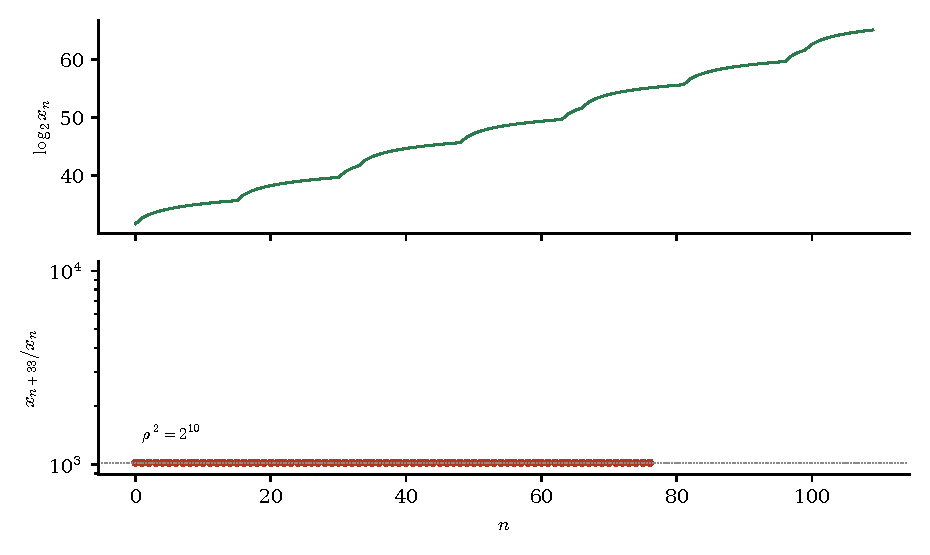
\includegraphics[width=0.97\linewidth]{figs/fig_scaling.pdf}
\caption{Exact asymptotic scaling for \(g=31\), single active prime \(2\). One class period has \(P=33\) steps and exponent increment \(5\), so \(x_{n+33}=2^{10}x_n=1024\,x_n\) for all \(n\) in the eventual regime. Left: the orbit \(\log_2x_n\) with the period marked; right: the ratio \(x_{n+33}/x_n\), exactly 1024 at every sampled \(n\).}\label{fig:scaling}
\end{figure}

\section{Which carries occur}

\begin{theorem}[Window theorem]\rec{F.T52}\scope{C}\label{thm:window}
In a persistent orbit with modulus \(g\):
\begin{enumerate}[label=(\alph*),nosep]
\item if \(g\) is odd then \(2\mid L_n\) for all \(n\);
\item if \(g\) is odd then \(g\nmid\gamma_n+1\) for all \(n\); if \(g\ge4\) is even then \(4g\nmid\gamma_n+1\);
\item every complete carry (Theorem~\ref{thm:carrycomp}) has \(M^2<g\) for odd \(g\) and \(M^2<4g\) for even \(g\); and \(\gcd(M,g)=1\).
\end{enumerate}
\end{theorem}
\begin{proof}
(a) is Lemma~\ref{thm:G-odd}. (b) If \(g\mid w\) with \(g\) odd then \(h=g\), \(b'=1\), and \(x'=(w/g)L^2\) is an integer. By Theorem~\ref{thm:onestep}, \(\Dx(x')=\{\text{all divisors}\ge2\text{ of }\sigma'\}\ni2\) by (a), and \(2\not\equiv1\ (\mathrm{mod}\ g)\), so \(x'\) is not persistent. For even \(g\) with \(4g\mid w\): \(\vv_2(w/g)\ge2\), so \(2\mid\sigma'\), \(b'=1\), and again \(2\in\Dx(x')\), \(2\not\equiv1\ (\mathrm{mod}\ g)\). (c) A complete carry starts from \(\gamma=1\) and passes through \(w=2,\dots,M^2\); by (b) the value \(w=g\) (resp. \(4g\)) is forbidden, so \(M^2<g\) (resp. \(<4g\)). \(\gcd(M,g)=1\) because \(M\mid d\equiv1\ (\mathrm{mod}\ g)\).
\end{proof}

\emph{Consequence.} A \(q\)-carry needs \(g>q^2\) (\(g\) odd). There are only finitely many carry sizes for a given \(g\) (all \(M<\sqrt g\)); 5-carries do not exist for odd \(g\le25\), 7-carries not for odd \(g\le49\).

\begin{theorem}[Absorption criterion]\rec{F.T53}\scope{C}\label{thm:absorb}
Let \((g,E)\) be a persistent state and \(w=\gamma+1\). For \(d\ge2\) with \(d\equiv1\ (\mathrm{mod}\ g)\) put \(j_p(d)=\max(0,\vv_p(d)-e_p)\) and \(M(d)=\prod_pp^{j_p(d)}\) (the \emph{new part} of \(d\)). Then \(d\) is available at the step iff \(M(d)^2\mid w\), and
\[
L'=L\cdot r,\qquad r=\mathrm{lcm}\{M(d):\ d\equiv1\ (\mathrm{mod}\ g),\ d\ge2,\ M(d)^2\mid w\}.
\]
\end{theorem}
\begin{proof}
By Theorem~\ref{thm:onestep}, \(d\mid\sigma'\) iff for all \(p\), \(j_p(d)\le\lfloor\vv_p(w/h)/2\rfloor\), iff \(M(d)^2\mid w/h\), iff \(M(d)^2\mid w\) (as \(h\mid g\) is coprime to \(M(d)\), since \(\gcd(d,g)=1\)). Persistence supplies \(d\equiv1\ (\mathrm{mod}\ b')\Rightarrow d\equiv1\ (\mathrm{mod}\ g)\), so availability does not depend on \(h\). The exponent of \(p\) in \(L'\) is \(\max(e_p,\max_d\vv_p(d))=e_p+\max_dj_p(d)\).
\end{proof}

A step is of \emph{no-absorption} type if no available \(d\) has \(M(d)>1\) (\(r=1\), \(\gamma'=\gamma+1\)); \emph{partial} if \(r>1\) and \(r^2<w\) (\(\gamma'=w/r^2\ge2\)); \emph{complete} if \(r^2=w\) (\(\gamma'=1\)). A complete carry has \(h=1\): indeed \(r^2\le s'^2\le w/h\), so \(w=r^2\le w/h\) forces \(h=1\).

\begin{theorem}[Carry completeness]\rec{F.T54}\scope{C}\label{thm:carrycomp}
Let a carry occur at \(w\) from a plateau that started at \(\gamma_s\) (the value of \(\gamma\) right after the previous carry, or the initial value). Then
\[
\gamma'\le\gamma_s/4+1,\qquad\text{and if }\gamma_s=1:\quad w=M^2=r^2\ \text{and}\ \gamma'=1\ (\text{complete}).
\]
Hence in a persistent orbit \(\gamma_s\) strictly decreases at every carry as long as \(\gamma_s\ge2\); after finitely many carries \(\gamma=1\), and from then on every carry is complete, \(w=M^2\), with cycle length \(M^2-1\).
\end{theorem}
\begin{proof}
\(L\) is constant along the plateau, so by Theorem~\ref{thm:absorb} availability of \(d\) depends only on \(M(d)^2\mid w\). Let \(d\) be available at the carry step. If \(w-M(d)^2\ge\gamma_s+1\), then \(d\) was already available at the earlier plateau step \(w''=w-M(d)^2\) (since \(M(d)^2\mid w''\)), i.e. the plateau would have ended there: a contradiction. So \(w\le\gamma_s+M(d)^2\). Since \(r\) is a multiple of \(M(d)\) and \(r\ge2\),
\[
\gamma'=\frac w{r^2}\le\frac{\gamma_s+M(d)^2}{r^2}\le\frac{\gamma_s}4+1.
\]
If \(\gamma_s=1\): \(M^2\mid w\) and \(M^2\le w\le1+M^2\) give \(w=M^2\) (since \(2M^2>M^2+1\)); then \(r^2\mid M^2\) and \(r\ge M\) give \(r=M\), \(\gamma'=1\). The last assertion: \(\gamma_s\ge2\) gives \(\gamma'\le\gamma_s/4+1<\gamma_s\), and \(\gamma_s\) is a positive integer; plateaus are finite and carries infinite by Theorem~\ref{thm:T47}.
\end{proof}

So the cycle \(1,2,3\) of regime~I is the case \(M=2\) of a general law: the \(\gamma\)-cycle is \(1,\dots,M^2-1\) with \(M\) the minimal available carry.

\begin{theorem}[Eventual carries are prime powers]\rec{F.T55}\scope{C}\label{thm:primepower}
In the eventually periodic regime every carry \(M\) is a prime power \(p^j\).
\end{theorem}
\begin{proof}
A carry type that recurs infinitely often raises each of its primes' exponents infinitely often, so each prime \(p\mid M\) has \(e_p\ge o_p-1\) (saturated) from some time on. Suppose \(M\) has two distinct primes and let \(d\) be available with \(M(d)=M\) (so \(w=M^2\), Theorem~\ref{thm:carrycomp}). Take a prime \(q\mid M\) with \(\vv_q(M)=j\). Choose \(i\in[0,o_q-1]\) with \(i\equiv e_q+j\ (\mathrm{mod}\ o_q)\); since \(e_q\ge o_q-1\), \(i\le e_q\). Then \(d'=d\,q^{i-e_q-j}\) is an integer, \(d'\equiv d\equiv1\ (\mathrm{mod}\ g)\), \(d'\ge2\) (it still contains the other prime of \(M\)), and \(M(d')=M/q^j<M\) with \(M(d')^2\mid M^2=w\). So a smaller carry was already available at \(w'=M(d')^2<M^2\), contradicting that the plateau reached \(w=M^2\).
\end{proof}

Composite carries (for example \(M=6\), \(w=36\)) occur only in the transient, while some participating prime is unsaturated.

\begin{theorem}[Odometer law]\rec{F.T56}\scope{C}\label{thm:odometer}
In the eventual regime let \(\mathcal P\) be the set of \emph{active} primes (unbounded exponent; all saturated) and call the others \emph{inert} (constant exponent). For \(p\in\mathcal P\) define
\[
\Abs_p=\{k\bmod o_p:\ \exists a\in\mathcal A_{-p},\ p^ka\equiv1\ (\mathrm{mod}\ g)\},
\]
where \(\mathcal A_{-p}\) is the set of residues of divisors of \(\prod_{q\ne p}q^{e_q}\) (\(\langle q\rangle\) for active \(q\); a fixed finite set for inert \(q\)). \(\Abs_p\subseteq\Z/o_p\) is time-independent. At every state with \(\gamma=1\), the next carry is \(p^{j_p}\) for the active \(p\) minimising \(p^{j_p}\), where
\[
j_p=\min\{j\ge1:\ (e_p+j)\bmod o_p\in\Abs_p\}.
\]
For a single active prime \(p\) the carry exponents are the successive gaps of \(\Abs_p\) around \(\Z/o_p\), the \(\gamma\)-cycle lengths are \(p^{2j}-1\), and over one lap \(P=\sum_i(p^{2j_i}-1)\) and \(\rho=p^{\sum_ij_i}\).
\end{theorem}
\begin{proof}
By Theorem~\ref{thm:carrycomp} the next carry from \(\gamma=1\) is the smallest \(M\) available at \(w=M^2\); by Theorem~\ref{thm:primepower} it is a prime power; and \(p^j\) is available iff \(p^{e_p+j}a\equiv1\) for some \(a\in\mathcal A_{-p}\) (no other prime has a new part). \(\mathcal A_{-p}\) does not change in time, so \(\Abs_p\) is fixed.
\end{proof}

\begin{example}[\(g=31\), \(p=2\)]\label{ex:g31}
Here \(o=5\) and \(\Abs=\{0,2,4\}\), with gaps \(2,2,1\). The carries are \(2^2,2^2,2^1\) (\(w=16,16,4\)), so \(P=15+15+3=33\) and \(\rho=2^5=32\); thus \(x_{n+33}=1024x_n\) (Figure~\ref{fig:scaling}). For \(g=59\) the carries are mostly \(3\)-carries (\(w=9\)) with occasional \(4\)-carries (\(w=16\)). The wheel of Figure~\ref{fig:wheel} shows \(\Abs\) as marked positions on \(\Z/o_p\).
\end{example}

\begin{figure}[t]
\centering
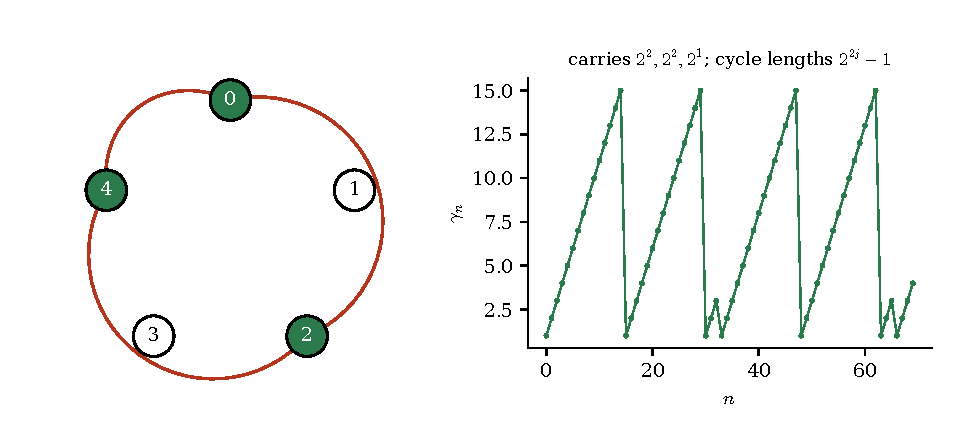
\includegraphics[width=0.62\linewidth]{figs/fig_wheel.pdf}
\caption{The odometer of Theorem~\ref{thm:odometer} for \(g=31\), \(p=2\): the exponent \(e_p\bmod5\) moves around the wheel \(\Z/5\); positions in \(\Abs=\{0,2,4\}\) are marked, and each carry advances the pointer to the next marked position. The gaps \(2,2,1\) are the exponents of the carries \(2^2,2^2,2^1\).}\label{fig:wheel}
\end{figure}

There is no other kind of eventual cycle: every eventual cycle of a persistent orbit is a word in prime-power carries generated by independent odometers. Chapter~\ref{ch:schedule} shows that in fact only one odometer runs.

\section{\texorpdfstring{The \(q\)-carry family}{The q-carry family}}

\begin{theorem}[The \(q\)-carry theorem]\rec{F.T57}\scope{C}\label{thm:qcarry}
Let \(q\) be an odd prime and \(g\) an odd prime with \(g>q^2\). Put \(o=\ord_g(q)\), \(H=\langle q\rangle\le(\Z/g)^\times\). Assume
\begin{itemize}[nosep]
\item[(Q1)] \(2\notin H\); let \(e_2=\min\{e\ge1:2^e\in H\}\) and \(K=\langle2\rangle H\);
\item[(Q2)] for every odd \(M\) with \(3\le M\le q-1\), \(M\bmod g\notin K\); for every even \(M\) with \(2\le M\le q-1\), \(M\bmod g\notin H\);
\item[(Q3)] \(u\) is a prime with \(u\equiv q\ (\mathrm{mod}\ g)\), \(u>q\); seed exponents \(E_0=\{u:o-1,\ q:\ge1,\ 2:e_2\}\);
\item[(Q4)] \(G(x_0)=g\) for \(x_0=L_0^2/g\), \(L_0=u^{o-1}q^{e_q}2^{e_2}\) (an exact, finite divisor check).
\end{itemize}
Then the orbit of \(x_0\) is persistent forever and
\begin{enumerate}[label=(\roman*),nosep]
\item \(\gamma_n=(n\bmod(q^2-1))+1\) and \(L_{n+q^2-1}=qL_n\); hence \(x_{n+q^2-1}=q^2x_n\);
\item every carry is the \(q\)-carry at \(w=q^2\), and every other step has \(r=1\);
\item \(R(x_n)=2e_q(n)+1\): it grows by 2 per carry.
\end{enumerate}
\end{theorem}
\begin{proof}
Induction on the carries. State: \(\gamma\) and exponents \((e_u,e_q,e_2)=(o-1,e,e_2)\), \(e\ge1\). All \(w\le q^2\) are \(<g\), so \(h=1\), \(b'=g\), and persistence is automatic from Theorem~\ref{thm:onestep} once all \(d\equiv1\ (\mathrm{mod}\ g)\). The residues of the \(u\)-part and \(q\)-part together make up \(H\) (\(u^c\equiv q^c\), \(c\in[0,o-1]\)), independent of \(e\). The only other prime is 2 with exponent \(e_2\ge1\) (no other prime has \(p^2\mid w\), since the primes below \(q\) have exponent 0 and \(u>q\)).

\emph{Available new parts at \(w<q^2\).} A new part \(M(d)=M\) has \(M^2\mid w<q^2\), so \(M\le q-1\), a product of primes \(<q\). If \(M\) is odd, 2 is not in \(M\), the 2-part ranges over \(2^0,\dots,2^{e_2}\) (which represent all of \(\langle2\rangle\) modulo \(H\)), and \(d\equiv1\) needs \(M\in\langle2\rangle H=K\): excluded by (Q2). If \(M\) is even, the 2-exponent is exactly \(e_2+j\) with \(2^{e_2}\in H\), and \(d\equiv1\) needs \(M\in H\): excluded by (Q2) (and \(2\notin H\) by (Q1) covers \(M=2\)). So \(r=1\) at every \(w\le q^2-1\).

\emph{At \(w=q^2\).} \(\sigma'=qL\); the new part \(M=q\) is available iff \(q^{e+1}u^c(2\text{-part with }2^a\in H)\equiv1\) for some \(c\le o-1\), i.e. \(q^{e+1+c}\equiv1\): \(c\equiv-(e+1)\ (\mathrm{mod}\ o)\) works. No other new part has \(M^2\mid q^2\). So \(r=q\), \(\gamma'=q^2/q^2=1\). The state after the carry has the same shape with \(e\to e+1\), proving (i) and (ii). For (iii): \(d=2^aq^bu^c\equiv1\) forces \(2^a\in H\), i.e. \(a\in\{0,e_2\}\) (\(2\notin H\) and \(e_2\) is the first return); for each \((a,b)\) there is exactly one \(c\bmod o\); so \(R+1=2(e+1)\).
\end{proof}

\emph{Instances} (verified by direct iteration of \(C\) and by a class-closure certificate, Theorem~\ref{thm:closure}): \(q=3\): \(g=11\) (seed \(\{47:4,3:1,2:2\}\); the orbit of Theorem~\ref{thm:eight} is a different saturator, \(5\equiv3^3\)), \(P=8\), \(\rho=3\); \(q=5\): \(g=31\), \(P=24\), \(\rho=5\); \(q=7\): \(g=367\), seed \(\{3677:60,7:1,2:3\}\), \(P=48\), \(\rho=7\), class period 2928, \(G=367\) exact. The smallest admissible \(g\) for \(q=3,5,7\) is \(11,31,367\).

\emph{Sharpness of (Q2).} It is necessary in the template: for \(g=193\), \(q=7\), the orbit is a 3-carry instead, because \(3\in\langle2\rangle H\) although \(3\notin H\).

\begin{example}[An even persistent value]\label{ex:68}
For \(g=68\) there is a persistent orbit, started at the reset state \((g,\gamma,E)=(68,1,\{3:3,\,13:1,\,3947:8,\,281:4\})\); verified by direct iteration of \(C\) and by class closure (Theorem~\ref{thm:closure}). So persistence is not restricted to odd \(g\): for even \(g\) the lcm \(L\) is odd, the collapse modulus is \(4g\), and the same carry calculus (Theorems~\ref{thm:onestep}--\ref{thm:odometer}) applies with \(M^2<4g\).
\end{example}

\begin{remark}[Scope of the earlier uniform statements]\rec{F.T58}\scope{C}\label{rem:T58}
The statements that every orbit is eventually \(x_{n+3}=4x_n\), or eventually of the form \(s^2t/g\) with \(t\in\{1,2,3\}\), are true for the regimes of Chapter~\ref{ch:regimes} and Theorems~\ref{thm:Pg}--\ref{thm:Pstar} and are not universal (Theorem~\ref{thm:eight}; the \(t\)-coordinate runs through \(1,\dots,q^2-1\) in Theorem~\ref{thm:qcarry}). The precise identity is, for \(G\) unchanged over three steps and \(x=\gamma L^2/g\),
\[
x_{n+3}=4x_n\iff\gamma_{n+3}L_{n+3}^2=4\gamma_nL_n^2\iff\gamma_{n+3}=4\gamma_n/\rho^2,\ \ \rho=L_{n+3}/L_n\in\Z_{\ge1}.
\]
The pairs \((\rho,\gamma_{n+3})=(2,\gamma_n)\) and \((1,4\gamma_n)\) are sufficient; other pairs with \(\rho^2\mid4\gamma_n\) are also allowed. The \(\gamma\)-cycle is \(1,\dots,M^2-1\) with \(M\) the minimal available prime-power carry (Theorem~\ref{thm:carrycomp}); \(M=2\) gives \(1,2,3\). Theorem~\ref{thm:T47} is consistent with all of this (\(\gamma\le8\le2M\) for the \(g=11\) orbit).
\end{remark}
